\documentclass{article}

% Language setting
% Replace `english' with e.g. `spanish' to change the document language
\usepackage[english]{babel}

% Set page size and margins
% Replace `letterpaper' with`a4paper' for UK/EU standard size
\usepackage[a4paper,top=2cm,bottom=2cm,left=3cm,right=3cm,marginparwidth=1.75cm]{geometry}
\usepackage{float}
\usepackage{lmodern}
\usepackage{scrextend}
\changefontsizes[18pt]{14pt}

% Useful packages
\usepackage{amsmath}
\usepackage{amsfonts} 
\usepackage{graphicx}
\usepackage[colorlinks=true, allcolors=blue]{hyperref}

\title{Central limit theorem}
\author{Matteo Bianchi}

\begin{document}
\maketitle

\begin{abstract}
Statistics project for the course of statistics of Cybersecurity at Sapienza.
I choose the Central limit theorem and in particular i concentrate my analysis  on  history, motivation,intuition and  all the math details behind the theorem
\end{abstract}

\section{Introduction}
\subsection{What is the central limit theorem}
In probability theory, the central limit theorem (CLT) states that the distribution of a sample variable approximates a normal distribution (i.e., a “bell curve”) as the sample size becomes larger, assuming that all samples are identical in size, and regardless of the population's actual distribution shape.

Put another way, CLT is a statistical premise that, given a sufficiently large sample size from a population with a finite level of variance, the mean of all sampled variables from the same population will be approximately equal to the mean of the whole population. 
Furthermore, these samples approximate a normal distribution, with their variances being approximately equal to the variance of the population as the sample size gets larger, according to the law of large numbers.
\subsection{Who discovered it}
The history of the Central limit theory is long and complicated animated by 2 century of mathematician.

The standard version of the central limit theorem was first proved by the French mathematician Pierre-Simon Laplace in 1810, states that the sum or average of an infinite sequence of independent and identically distributed random variables, when suitably rescaled, tends to a normal distribution.

Fourteen years later the French mathematician Siméon-Denis Poisson began a continuing process of improvement and generalization.
Laplace and his contemporaries were interested in the theorem primarily because of its importance in repeated measurements of the same quantity. If the individual measurements could be viewed as approximately independent and identically distributed, then their mean could be approximated by a normal distribution.
Then Peter Gustav Lejeune Dirichlet (1805–1859) prove the theorem in 1846
but it was not until the nineteenth century was at an end that the importance of the central limit theorem was discerned, when, in 1901, Russian mathematician Aleksandr Lyapunov defined it in general terms and proved precisely how it worked mathematically.
Nowadays, the central limit theorem is considered to be the unofficial sovereign of probability theory.


\section{History of the CTL }

\subsection{Discovery of the normal curve: Chapter 0 of the CLT}
The normal curve is perhaps the most important probability graph in all of statistics.
Its formula is 
\[  y=\frac{1}{\sqrt{2\pi}\sigma}e^{-\frac{1}{2}(\frac{x-\mu}{\sigma})^2  }   \]

 Where the  “e”  is the irrational number we use as the base for natural logarithms. $ \mu $ and $ \sigma $ are
the mean and standard deviation of the curve

\subsubsection{Abram De Moivre Discoveries}
De Moivre pioneered the development of analytic geometry and the theory of probability by expanding upon the work of his predecessors, particularly Christiaan Huygens and several members of the Bernoulli family. He also produced the second textbook on probability theory.He was a consultant for  gamblers, in fact he derive the formula trying to  solving a gambling
problem whose solution depended on finding the sum of the terms of a binomial distribution. Later work,especially by Gauss about 1800, used the normal distribution to describe the pattern of random
measurement error in observational data. Neither man used the name “normal curve.” That expression did not appear until the 1870s.


The normal curve formula appears in mathematics as a limiting case of what would happen if you had an
infinite number of data points. To prove mathematically that some theoretical distribution is actually
normal you have to be familiar with the idea of limits, with adding up more and more smaller and smaller
terms. This process is a fundamental component of calculus. So it’s not surprising that the formula first
appeared at the same time the basic ideas of calculus were being developed in England and Europe in the
late 17th and early 18th centuries.

the normal curve formula first appeared in a paper by DeMoivre in 1733. He lived in
England, having left France when he was about 20 years old. Many French .
Protestants, the Huguenots, left France when the King canceled the Edict of Nantes
which had given them civil rights. In England DeMoivre became a good friend of
Isaac Newton and other prominent mathematicians.
He wrote the 1733 paper in Latin, and in 1738 he translated it himself into English for
the 2nd edition of his book, The Doctrine of Chances, one of the first textbooks on
probability. (The first edition had been published in 1718.)
In DeMoivre’s work the normal curve formula did not look like it does now, in particular because there
was no notation then for e. and there was no general sense of standard deviation, which is represented by $ \sigma $ in today’s equation.

\subsubsection{Why did DeMoivre do it? What problem was he working on?}

He is dealing with “Problems of Chance,” that he wants
to see how likely it is that an
“experiment” will produce a given
outcome. Note that he credits the
Bernoulli brothers with prior work –
but they just didn’t do quite enough.
The core problem for DeMoivre is to
find the sum of “several” terms in a
binomial expansion. He wanted a
shortcut because the problem was “so
laborious.”
DeMoivre wanted to avoid having to add up all these coefficients. He needed to describe the general
shape of the distribution of the values on a line of coefficients without having to compute each one. We can see what happens with a few graphs.
A clear example of this problem can be seen in:
\begin{table}[H]
\centering
\begin{tabular}{c|c|c|c}
    n &  Expansion of $ (a+b))^n $ & Coefficients & Sum $ 2^{n} $ \\\hline

    1 &  a+b& 1 1 & 2                                \\
    2 & $ a^2 +2ab+b^2 $ & 1 2 1 & 4                     \\
    3 & $ a^3+3a^{2}b+3ab^2+b^3 $ & 1 3 3 1 & 8                \\
    4 & ---   & 1 4 6 4 1 & 16                         \\
    5 & ---   & 1 5 10 10 5 1 & 32                     \\
    - & etc. & etc. & etc.                         \\

\end{tabular}
\caption{\label{tab:widgets}Coefficients table}
\end{table}

Imagine that you want to find the sum of
several terms in one line, say the middle two
terms in line for n = 5.
We quickly see that 10 + 10 = 20.
But what if you want to find the sum of the middle
10 terms in the line where n = 100? A problem like
this could easily come up in a game of chance. This
is what he meant by “laborious.”

DeMoivre wanted to avoid having to add up all these coefficients. A solution is to describe the general shape of the distribution of the values on a line of coefficients without having to compute each one. We
can see(as he noticed) that as number of event increase distribution approached a smooth curve.

ex. Lets start with a binomial distribution for two event
\begin{figure}[H]
\centering
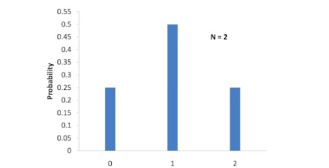
\includegraphics[width=0.5\textwidth]{images/0.png}
\caption{\label{fig:bin2}Binomial distribution of two event.}
\end{figure}

Then adding more event

\begin{figure}[H]
\centering
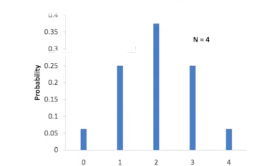
\includegraphics[width=0.5\textwidth]{images/1.png}
\caption{\label{fig:bin4}Binomial distribution of 4 event.}
\end{figure}
Then looking for a more crowded situation
\begin{figure}[H]
\centering
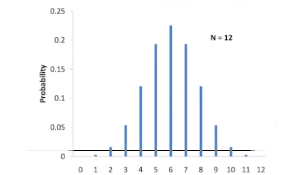
\includegraphics[width=0.5\textwidth]{images/2.png}
\caption{\label{fig:bin12}Binomial distribution of 12 event.}
\end{figure}

De Moivre understand the important of this result and try to find a way to write this curve
infact if you can replace the binomial coefficient graph that is made up of lots of bars by a smooth curve, then
instead of having to add lots of individual numbers you can just find the area under the curve, which is
exactly one of calculus’s strengths. You can see that as n increases the graphs look more and more like a
bell-curve.
DeMoivre began by considering the expansion of $ (1+1)^{n} $ . This expression comes up naturally in
analyzing a coin toss with equal probabilities of heads and tails. He focused on the ratio of the middle
term to the sum of all the coefficients, $ 2^n $ .
DeMoivre wanted to know what happens to the ratio when n gets very large. It is informative to see how a 17th century mathematician has to deal with such a problem.
He had “a dozen years or more” ago found that the ratio of the middle term to the sum can be expressed, using modern parentheses, as  $ R= 2A(n+1)^{n} / n^{n} \sqrt{n-1} $.

He wants to determine the value of R for any given n. Once he gets that, he knows the height of the curve at the middle and could then build the rest from that. He used some results he had found earlier about limits, some earlier work by James Bernoulli, and work that James Stirling did at just the right time to help.

First DeMoivre rewrites his fraction as   $ R= 2A/ \sqrt{n-1} * (1-(1/n))^{n} $.

Then since he wants to find the limiting value of this expression when n approaches infinity (Many mathematicians of that time were working on problems that involved expanding binomial expressions) he uses the earlier work by James Bernoulli to say that the limit for $ (1-(1/n))^{n} $ is “the number
whose hyperbolic logarithm is -1.” Today we say “natural” logarithm instead of hyperbolic logarithm,and we would therefore write $ \lim_{n\to\infty}  (1-(1/n))^{n}  = e^{-1}  $.
so for large value of n we car replace th limit with $ e^{-1} $
That gets us to the ratio as $ R=  \frac {2Ae^{-1}}{\sqrt(n-1)} $
He also states that he has shown in his own earlier work that A is the number whose hyperbolic logarithm is $ \frac{1}{12} - \frac{1}{360} + \frac{1}{1260} - \frac{1}{1680} + ...  $  or in modern notation $ e^{....} $
So doing some math we can rewrite R as $ \frac{2}{(e^{ \frac{1}{12} - \frac{1}{360} + \frac{1}{1260} - \frac{1}{1680} + ... }) \sqrt{n-1}  } $

DeMoivre called the messy looking part B. So he ends up with $ R= \frac{2}{B \sqrt{n-1}} $
DeMoivre says this is as far as had gotten when he had last worked on the problem.
It had been good enough for him to do some approximate calculations but he did not get a “nice” expression for B.
Lucky for him, his friend and colleague,
James Stirling, showed the exact value of B.
Since the circumference of a circle whose radius is 1 is $ \pi $, we can write DeMoivre’s formula for the desired ratio as R = $ \frac{2}{ \sqrt{2\pi}\sqrt{n-1} } $.
Then he reasoned that for really large values of n there’s no appreciable difference between $ \sqrt{n-1} $ and  $ \sqrt{n}$.
We can therefore write the ratio as  R = $ \frac{2}{ \sqrt{2\pi}\sqrt{n} } $.
This starts to look like the modern formula for the normal curve.
We can show the similarity further remembering that DeMoivre is approximating a binomial with $ p= \frac{1}{2} $. The standard deviation for a binomial distribution is given by $ \sigma = \sqrt{np(1-p)} $ and replaced p with $ \frac{1}{2} $  get us to $ \sigma = \frac{ \sqrt{n}}{2} $.
Solving this for $ \sqrt{n}$ we get $ \sqrt{n}= 2\sigma $.
And so finally R= $ \frac{1}{\sqrt{2\pi}\sigma}$
This is exactly the y value of the normal curve at the center where x = $ \mu $.
$ y= \frac{1}{\sqrt{2\pi}\sigma }e^{{\frac{-(x-\mu)^{2}}{2\sigma^{2}}}}=  \frac{1}{\sqrt{2\pi}\sigma} $

\subsection{Some statistical consequences.}
The formula itself would be found to have more and more applications, beyond just the approximation of a binomial distribution, especially as a model for the distribution of random measurement errors. Also,equally informative, the relationship $ \sigma = \frac{\sqrt{n}}{2}$, shows that the narrowness of the normal curve, as measured by $\sigma$, is proportional to the square-root of the sample size. This implies, for example, that if you wish to cut a margin of error in half, you will need four times as much information, not twice as much. Another way to say this is that the information you gain in collecting data is proportional, not to the number of pieces of data, but to its square root.

De Moivre’s approximations to binomial distributions did not do justice to the universality that characterizes the CLT. For the sake of completeness, but also to demonstrate what tremendous progress Laplace’s approximations of 1810 represented, de Moivre’s 1733 paper should be recognized as a sort of “0th chapter,” as it were, in the history of the CLT.

\subsection{Gauss}
Gauss about 1800, used the normal distribution to describe the pattern of random measurement error in observational data. Neither man used the name “normal curve.” That expression did not appear until the 1870s.

\subsection{The Central Limit Theorem from Laplace to Cauchy }
in 1812, Pierre-Simon de Laplace (1749–1827) published the first edition of his
Théorie analytique des probabilités (henceforth simply abbreviated by TAP).1 With
its typical problems, stochastic models, and analytic methods this book would considerably influence probability theory and mathematical statistics right until the beginning of the 20th century.\cite{Fischer2010History}
Until Laplace and his successors, classical probability consisted mainly in the
sum of its applications to physical, social, and moral problems. However, as Laplace
already pointed out in the concise preface to the first edition of his TAP, probability
was also important for mathematics in a narrower sense. In many problems referring
to stochastic models depending on a large number of trials, probabilities could only
be expressed by formulae too complicated for direct numerical evaluation. Thus,
for a reasonable application of many of the results of probability calculus, particular considerations were needed to obtain useful approximations of the “formulae
of large numbers.” In the aforementioned preface, Laplace called these problems
“the most delicate, the most difficult, and the most useful” of the entire theory.
He expressed his hope that discussion of these problems would catch the attention of
other “geometers.” Therefore, in addition to the qualitative feature of applicability,
which was characteristic for classical probability theory, a new, purely mathematical
aspect emerged: the relevance of specific analytical methods of probability theory.
Laplace had been intensely dealing with the “delicate problems” of probability
just described from the very beginning of his scientific career. In his 1781 “Mémoire
sur les probabilités,” one can already find “in nuce” almost all of the problems of
TAP, which can be roughly divided into two categories: “sums of random variables”
and “inverse probabilities.”2 The first category includes, for example, the a priori
probabilities of profit and loss in certain games of chance, or of the arithmetic mean
of observations being subject to random errors; the latter for instance deals with the
a posteriori probabilities that the ratio of the chances of a boy’s and a girl’s birth
is within a given interval centered around the ratio of the corresponding observed
values. By 1774, Laplace had already developed useful approximation methods for
those a posteriori probabilities depending on a large number of observations. He did
not succeed in adapting this method to a priori probabilities until 1810, however.
Only then, with a “tricky” modification of the method of generating functions, did
he achieve any usable results on approximations of probabilities of sums of independent random variables, which, from the modern point of view, are subsumed under
the rubric of the “central limit theorem.” It was the CLT which considerably shaped
the contents and methods of the TAP and significantly influenced the development
of probability and error theory during the 19th century.
The history of the CLT, as far as the contributions of Laplace and his successors are concerned, has already been studied in
fair detail. Therefore, a main focus in the present section will be on those questions
which still seem to be open: Which changes in the probabilistic and analytical context of the CLT occurred between ca. 1810 and 1850; how did these changes come
about, and how have these changes influenced analytical style and methods in the
treatment of this theorem?
\subsection{Laplace’s Central “Limit” Theorem}
As already noticed, Laplace’s CLT was the result of an almost forty years’ effort.
In the following, we will describe the historical development of Laplace’s treatment
of sums of independent random variables, his methods for finding appropriate approximation formulae, and the major applications of his finally achieved CLT.
\subsubsection{Sums of Independent Random Variables}
Sums of independent random variables had played an important role in Laplace’s
probabilistic work from the very beginning.3 In this context, the problem of calculating the probability distribution of the sum of angles of inclination, which were
assumed to be determined randomly, as well as the related problem of calculating
the probabilities of the deviations between the arithmetic mean of data which were
afflicted by observational errors and the underlying “true value,” became especially
important. In one of his first published papers, Laplace \cite{Fischer2010History} had already set out to
determine the probability that the sum of the angles of inclination of comet orbits (or
the arithmetic mean of these angles respectively) is within given limits. He assumed
that all angles, which had to be measured against the ecliptic, were distributed randomly according to a uniform distribution between 0ı and 90ı (and also tacitly
presupposed that all angles were stochastically independent). Laplace succeeded in
calculating these probabilities for an arbitrary number of comets via induction (with
a minor mistake which was subsequently corrected in \cite{Laplace2012Pierre}).
In this paper ( Original released in 1781 ) paper, Laplace even introduced a general—however very intricate—method, based
on convolutions of density functions, in order to exactly determine the probability
that a sum of independent random variables (“quantités variables,” as Laplace put it)
was within given limits.In the most simple case, each of the n variables had the
same rectangular distribution between 0 and h. For the probability P that the sum
of those variables was between a and b with $ 0 \leq a< b \leq nh $ , Laplace obtained (in
modern notation)
$ P= \frac{1}{h^{n}n!}(\sum\limits_{n=0}^{N}\binom{n}{i}(-1)^{i}(b-ih)^{n}- \sum\limits_{i=0}^{M}\binom{n}{i}(-1)^{i}(a-ih)^{n}  ) $

where $ N= \min(n,[\frac{b}{h}]) $ and $ M= \min(n,[\frac{a}{h}])$.
Formulae of this kind were too complicated for a direct numerical evaluation if the number of random variables exceeded a relatively small value. The arithmetic mean of the actual observed angles of inclination of the then known 63 comets was $46^{\circ} 16^{\prime} $. Through the use of upper formula  alone, Laplace was unable to address the hypothesis that the comets’ planes of motion resulted at “random.” At this stage of his mathematical work, however,Laplace could not develop usable approximation.
Laplace infact developed techniques for approximating integrals depending on a "great number" such as the Gamma function in subsequent years.

\subsubsection{Deduction  of Approximating Normal Distributions}
Laplace for the first time exemplified his approach to the CLT in the “Mémoire
sur les approximations des formules qui sont fonctions des très grands nombres
et sur leur application aux probabilités” [1810]. Crucial for this success in
approximating distributions of sums of independent random variables by normal
distributions was his modification of generating functions.

Let me demonstrate the essentials of his approach to the CLT  in the special case of identically distributed
random variables X1 ; : : : ; Xn , which have zero means and which take the val-
ues $ \frac{k}{m}$(m a given natural number, k = -m,-m+1,...,m-1,m )with the
respective probabilities Pk .
For the calculation of the probability Pj that $ \sum_{l=1}^{n} X_{l} $ 
has the value m$\frac{j}{m}(-nm \leq j \leq nm)$, Laplace made use of the generating function:
\[ T(t) = \sum_{k=-n}^{m} Pk^{t^{k}} \]
Due to the mutual independence of the $X_l$ ’ which was usually only tacitly presupposed by Laplace $P_j$ is equal to the coefficient
of $ t^{j}  $ in $ [T(t)]^n  $  after carrying out the multiplication.
The direct execution of this method—its general principle going back to de Moivre, see [Seal 1949]—leads at
best to very complicated algebraic terms for $P_j$ .
Laplace, however, introduced the trick of substituting the variable t by $ e^{ix} (i= \sqrt{-1})$. Thus, he introduced the (now so-called) characteristic functions in a special case.

From:
  \[ \frac{1}{2\pi} \int_{-\pi}^{ \pi} e^{-itx} e^{isx} dx = \delta_{ts} (t,s \in \mathbb{Z} ) \]   
it follows that:
  
  \[ P(j) = \frac{1}{2\pi} \int _{-\pi}^{\pi} e^{-ijx}[\sum_{k=-m}^{m} pke^{ikx}]^n dx. \] 
  The last integral above was at least formally accessible to Laplace’s method of approximation. There was, however, a certain modification necessary, as Laplace did not consider an expansion of the whole integrand around its maximum at
x = 0, but only of the power with exponent n (equal to the characteristic function).
By expanding $e^{ikx}$ into powers of x and taking into consideration that
$  \sum_{k=-m}^{m} pk^{k}= 0 $ and with the substitution $ m^2\sigma^2 = \sum_{k=-m}^{m} pk^{k^2}$,we obtain 
\[ P(j) = \frac{1}{2\pi} \int _{-\pi}^{\pi} e^{-ijx}[1-\frac{m^2\sigma^2x^2}{2} -iAx^3 + ... ]^n dx. \] where A is a constant depending on $ \sum_{k=-m}^{m} pk^{k^3}$.
The formal expansion of :
\[ log[1-\frac{m^2\sigma^2x^2}{2} -iAx^3 + ... ]^n = : log z \]
into a series of powers of x x leads to:
\[ log z= -\frac{m^2\sigma^2x^2}{2} -iAx^3 + ... , \]

and therefrom to
\[  z= e^{-\frac{m^2\sigma^2x^2}{2} -iAx^3 + ...}= e^{\frac{m^2\sigma^2x^2}{2}}(1-iAnx^3+...).   \]
After transforming the variable of integration according to $ x= \frac{y}{\sqrt{n}}$, the result is 
\[ P(j) = \frac{1}{2\pi\sqrt{n}} \int _{-\pi\sqrt{n}}^{\pi\sqrt{n}} e^{-ij\frac{y}{\sqrt{n}}}          e^{-\frac{m^2\sigma^2y^2}{2}}  ( 1 - \frac{iAy^3}{\sqrt{n}} + ...)  dy. \] For an approximation p with a “very large” n we ignore, like Laplace, all series terms  with a power of $ \sqrt{n}$ in the denominator, and at the same time, set the limits of integration equal to $\pm \infty$.   
In this way we get
\[ P(j) = \frac{1}{2\pi\sqrt{n}} \int _{- \infty}^{\infty}  e^{-ij\frac{y}{\sqrt{n}}}          e^{-\frac{m^2\sigma^2y^2}{2}}  dy. \]
where the last integral is, as Laplace showed in different ways, equal to:

\[  \frac{1}{m\sigma\sqrt{2\pi n}}e^{-\frac{j^2}{2m^2\sigma^2n}}  \]
Summing up this for $\frac{j}{m} \in [r1\sqrt{n};r2\sqrt{n}]$ , that can be approximated by integration $dx \approx \frac{1}{\sqrt{n}}$,leads to 

\[    P(r1\sqrt{n} \leq \sum X_l \leq r2\sqrt{n}) \approx \sum_{j\in[mr1\sqrt{n}; mr2\sqrt{n}]} \frac{1}{m\sigma\sqrt{2\pi n}} e^{-\frac{j^2}{2m^2\sigma^2n}} \approx \int_{r1}^{r2}\frac{1}{\sigma\sqrt{2\pi}}e^{-\frac{x^2}{2\sigma^2}} dx.  \]
which corresponds to the integral form of the CLT. With only one exception Laplace dealt with independent identically distributed and bounded
random variables with densities. 
To this aim he at first considered the range of values of those random variables discrete (as described above), and then he assumed m “infinitely large.”
Nowhere in his work did Laplace state a general theorem which would have
corresponded to the CLT in today’s sense.
He only treated particular problems concerning the approximation of probabilities of sums or linear combinations of a great
number of random variables (in many cases errors of observation)
by methods which in principle corresponded to the procedure described above.
In modern notation, Laplace’s most general version of the CLT 
was as follows: Let  $ \epsilon_1.....\epsilon_n$ be a large number of in-
dependent errors of observation, each having the same density with mean $\mu$ and
variance $ \sigma^2$ . If  $ \lambda_1 ... \lambda_n $ are constant multipliers and $a > 0$, then:
\[ P(|\sum_{j=1}^{n}\lambda_j(\epsilon_j -\mu)| \leq a \sqrt{\sum_{j=1}^n \lambda_j^2}  ) \approx \frac{2}{\sigma\sqrt{2\pi}}\int_0^a e^{-\frac{x^2}{2\sigma^2}} dx. \]
The special case of a CLT for the binomial distribution Laplace \cite{Laplace2012Pierre} on the basis of Stirling’s formula treated in a particular section of his TAP
by methods which are in principle due to de Moivre and still employed in modern textbooks. 


\subsection{Poisson’s Modifications}
Among all contributions of the 19th century in connection with Laplace’s CLT aiming at a more comprehensible presentation or at modifications of the Laplacian methods according to contemporary analytical standards, the two approaches \cite{Dodge2008Concise} by Siméon Denis Poisson (1781–1840) had a special influence on the contributions of later authors. 
Poisson shared Laplace’s view on the status of probability theory in the classical sense.
Concerning moral problems, however, Poisson generalized Laplace’s stochastic models to a considerable extent, and he did not share Laplace’s cautious attitude toward these issues. Poisson’s idea of all processes in the physical and moral world being governed by distinct mathematical laws is in line with his attempts toward a more exact mathematical analysis. 

Accordingly, the consequences for CLT were twofold: Firstly, Poisson formulated and proved this theorem generally for “choses,” thus creating an early concept of random variables, and secondly, he tried to discuss the validity of this theorem, mainly through counterexamples.
\subsubsection{Poisson’s Concept of Random Variable}
In the first \cite{Fischer2010History} of the above-mentioned articles, Poisson treated sums and linear
combinations of observational errors with different (not necessarily symmetrical)
distributions, followed by a discussion of the Laplacian foundation of least squares.
In the second article of 1829, he took up the issue from a far more general point of
view. There, Poisson investigated asymptotic behavior of the distribution of a sum
of functions (!) of the values of a “thing” (“chose”), where in several independent
experiments these values were obtained with possibly different probabilities. The
additional complication of considering a “function” essentially served to cover bothsums of random values and of powers of these values within the same theorem. 
From today’s point of view, all these quantities would plainly be described as random variables. Thus, Poisson’s concept of the values of a “thing” was directed primarily toward the most important applications, and was still far away from the modern conception of abstract “random variable,” as explained by Kolmogorov (1933).

\subsection{ Poisson Central Limit Theorem}
As we will see in the following, Poisson’s work on the CLT was based on Laplace’s ideas on the one hand; on the other hand, however, Poisson’s discussion of new analytical aspects paved the way toward a more rigorous treatment of the CLT.

\subsubsection{Poisson’s Version of the Central Limit Theorem}
Poisson’s results concerning the CLT can be summarized in modern terminology
essentially as follows:
Let $X_1,....,X_s $be a great number of independent random variables with density functions which decrease sufficiently fast (Poisson did not specify exactly how fast)as their arguments tend to $ \pm \infty$.
It is supposed that for the absolute values $\rho_n(\alpha) $ of the characteristic function of $X_n$ there exist a function $r(\alpha)$ indipendent of n with $ 0 \leq r(\alpha) < 1 $ for all $\alpha \neq 0$ such that $\rho_n (\alpha) \leq r(\alpha) $ Then, for arbitrary $ y,y' $:
\[   P(y\leq \frac{\sum_{n=1}^s(X_n - EX_n)  }{\sqrt{2\sum_{n=1}^s VarX_n}}   \leq y' )  \approx \frac{1}{\sqrt{\pi}} \int_y^{y'} e^{-u^2} du.  \]
where the approximation becomes all the better the larger s is, and the difference between the left and the right side becomes “infinitely small” with “infinite” s. Strictly speaking, Poisson’s analysis could be used for arbitrary y, y', though he explicitly expressed end results in the sense of (2.19) only for the special case y= -y' <0.
Poisson was convinced that this CLT was also valid for discrete random vari-
ables. In this case one could, according to Poisson \cite{Dodge2008Concise}, assume that the
values $c_1 ,....,c_v$of a random variable of this kind were subject to the respective
probabilities $y_1,....,y_v $ which were represented by $y_i = \int_{c_i -\delta}^{c_i +\delta} f(z)dz$
 with an “infinitely small” quantity $\delta$ and a “discontinuous” density function $f$.
As with Laplace, the CLT for Poisson was an important tool of classical probabil-
ity, but not an autonomous mathematical theorem. Unlike Laplace, however, Pois-
son pointed out essential presuppositions “en passant,” such as the above-mentioned condition  for characteristic functions, and he discussed counterexamples to an overall validity of asymptotic normal distributions for sums. The most prominent of these counterexamples \cite{Fischer2010History} concerns the sum of identically distributed random variables with the probability density:
\[f(x)= \frac{1}{\pi (1+x^2)}\]

or which the direct evaluation of  shows that:
\[P(c-\epsilon \leq \sum X_n \leq c+\epsilon ) = \frac{1}{\pi} arctan (\frac{2\epsilon s }{s^2 +c^2-\epsilon^2})\]
Therefore in this case, even for large s, an approximate normal distribution can
not be reached. Poisson \cite{Dodge2008Concise} pointed out, however, that such cases of very
slowly decreasing densities would not occur in practice, because all errors of observation were uniformly bounded in reality. Random variables with the density function f would later play an important role in Cauchy’s critical discussion of least squares . In fact, such random variables are now called “Cauchy-distributed.”
The significance of his condition for characteristic functions  Poisson illustrated by two similar examples, where neither the assertion
of the CLT was true nor this condition was met: He considered linear combinations $\sum_{n=1}^s y_n \epsilon_n$ of identicaly distributed errors obeying the law 
$f(x)= e^{-2|x|}$ . He showed that for an "infinitly large" s:
\[P(-c \leq \sum y_n \epsilon_n \leq c)  = \frac{1-e^{-2c}}{1+e^{2c}} if y_n = \frac{1}{n}, \]and: 

\[P(-c \leq \sum y_n \epsilon_n \leq c)  = 1- \frac{4}{\pi}arctan(e^{-2c})  \]\[ if    y_n = \frac{1}{2n-1}, \] 

According to Poisson, in the first example we have
\[   \rho_1(\alpha)...\rho_s(\alpha)= \frac{1}{(1+\frac{a^2}{4})(1+\frac{a^2}{4*4})...(1+\frac{\alpha^2}{4s^2})} \succ \frac{\pi \alpha}{e^{\frac{1}{2}\pi \alpha} -e^{-\frac{1}{2} \pi \alpha}}  \]
whereas in the second :

\[   \rho_1(\alpha)...\rho_s(\alpha) = \frac{1}{(1+\frac{a^2}{4})(1+\frac{a^2}{4*9})...(1+\frac{\alpha^2}{4 (2s-1)^2})} \succ \frac{2}{e^{\frac{\pi \alpha}{4}} -e^{-\frac{\pi \alpha}{4}}}  \]
\subsection{ Poisson’s Law of Large Numbers}
Regarding error theory, Poisson hardly made any modifications to the Laplacian
discussion of least squares based on the CLT. Yet the discussion of (in modern terms)stochastic convergence of mean values and relative frequencies,respectively, which did not play a too dominant role in Laplace’s work, became vital for Poisson and his major probabilistic work, the Recherches. Like Laplace, Poisson based such considerations on the CLT.

The approximate stability of arithmetic means or relative frequencies, quite often
observed within different sequences of random experiments of the same kind, was
so important for Poisson’s probabilistic approach that he coined the term “law of
large numbers” for this fact. In the introduction of his Recherches, he characterized this law as follows:

\textit{The phenomena of any kind are subject to a general law, which one can call the Law of Large Numbers. 
It consists in the fact, that, if one observes very large numbers of phenomena of the same kind depending on constant or irregularly changeable causes, however not
progressively changeable, but one moment in the one sense, the other moment in the other sense; one finds ratios of these numbers which are almost constant \cite{Fischer2010History}}.

It must be emphasized that Poisson’s interpretation of “law of large numbers” is
different from the modern definition of this term.

For a “proof” of his law of large numbers, Poisson introduced a special two-stage model of causation for the occurrence of an event
(or, more generally, for the occurrence of a special value of a “chose”), and he established two auxiliary theorems on stochastic convergence: 
the first concerning the arithmetic means of non-identically distributed random variables, the second concerning the relative frequencies of an event which generally does not occur with constant probability. 
He based these theorems, which are equivalent to the now so-called “laws of large numbers,” on his general CLT (for comprehensive historical accounts).

A distinct deviation of the relative frequencies with which a certain event had occurred in different sequences of observations respectively, possibly gave rise to the assumption that these sequences originated from different systems of causation. In the third part of his Recherches, Poisson gave a probabilistic discussion of the significance of such hypotheses in the context of conviction rates, and he essentially used the CLT for calculating the respective probabilities.

Poisson’s law of large numbers (in its original form) was heavily criticized during the 19th century. Among these discussions, two crucial points became subject of debates: the practical meaning of Poisson’s causation system was scrutinized (mainly by Bienaymé), and the analytical rigor of the deduction of the “auxiliary” CLT was questioned.

Chebyshev \cite{Remez1962General} criticized that Poisson’s analysis was only “approximative,”
and did not provide exact “error limits.”
In this way he showed a—still rather vague—unease with Poisson’s analytical approach. 
One can, however, interpret Chebyshev’s criticism as an indication of the shift from “classical” probability, chiefly determined by its applications, toward a “new mathematical” probability.

Perhaps, Chebyshev’s objections resulted from Poisson’s (as well as Laplace’s)
procedure of neglecting “higher” series terms without giving any justification for
that. Yet, if this was the case, Chebyshev did possibly not realize that Poisson had
given an—at least indirect—justification of this procedure with his first, infinitistic
approach.

\subsection{Proof}
\subsubsection{Dirichlet’s Modification of the Laplacian Method
of Approximation}
Dirichlet’s main probabilistic interests lay in problems of approximating “functions
of large numbers.” Thus, he actually satisfied Laplace’s hope that such questions
would interest the “geometers” (see the introductional part of the present chapter).
At the same time, one can see in Dirichlet’s activities a shift from the typical objects of classical probability, concentrating on practical applicability, toward the discus-sion of the respective analytical methods.

In the 1830s, Dirichlet presented Laplace’s original deduction of Stirling’s formula in his lectures.
He succeeded at least in deducing the law of Laplace’s series, which Cauchy \cite{1852Comptes} would still consider to be unknown

\subsubsection{ Dirichlet’s Proof}
Dirichlet’s discussion of the asymptotic distribution of linear combinations of
observational errors can be reconstructed in the sense of a rigorous proof of the
CLT, even from today’s point of view.
\subsubsection{Tacit Assumptions and Proposition}
As described above, Dirichlet discussed linear combinations $ \alpha_1x_1+ ... +\alpha_n x_n$ of
random errors.
The densities of these errors were not only considered to be symmetric and concentrated on a fixed interval, but also to be smooth (in the sense of the existence of continuous derivatives) and unimodal, as it appears from a picture in the lecture notes \cite{Hardy2013Dirchlet}. 
The latter assumption was, however, not absolutely necessary for Dirichlet’s deductions.

As we will see, Dirichlet tacitly presupposed that
the sequence of the, $\alpha_v$ had a positive lower bound (named $\alpha$ by me) and a positive upper bound (A), and that all variances of the random errors should be uniformly bounded away from 0 (by a positive lower bound to which I refer as k). Such tacit assumptions were natural within error theory. For a rigorous completion of Dirichlet’s line of proof in the case of non-identically distributed observation errors, one has to additionally assume a certain uniformity in the shape of all the density functions,such as, for example, the existence of an upper bound C such that $|f_v'(x)|< C $ for all $ x \in [-a;a] $ and all v. (From this condition one can already deduce the existence of the above-mentioned constant k.)
Expressed as a “modern” limit assertion, the main result of Dirichlet’s lecture
course on error theory in 1846 was:
\[ |P(-\lambda\sqrt{n} \leq \sum_{v=1}^n  \alpha_v x_v \leq \lambda \sqrt{n})-\frac{2}{\sqrt{\pi}}\int_0^{\lambda /r} e^{-s^2} ds|  \rightarrow  0 (n \rightarrow \infty)\]
where

\[r= 2 \sqrt{\frac{1}{n}\sum_{v=1}^n k_v \alpha_v^2 }\]
Even if the transcriber of the lecture notes did apparently not render all arguments
entirely correctly, the basic ideas for a rigorous proof of this limit can be clearly
discerned. At least in the special case of identically distributed errors a complete
argumentation can be reached with such methods that Dirichlet himself used.


\subsubsection{ Dirichlet’s Discussion of the Limit}
On the basis of his studies  we can reconstruct Dirichlet’s result by the inequality:
\[ | P(- \lambda \sqrt{n} \leq \sum_{v=1}^n \alpha_v x_v \leq \lambda\sqrt{n}  ) - \frac{2}{\sqrt{\pi}} \int_0^{\lambda/r} e^{-s^2} ds  |   \leq \lambda C_1(n) +C_2(n)+\lambda C_3(n) +C_4(n) \]
which is valid for asufficiently large n Presupposing 
\[ \delta = n^{-1/2 +\epsilon}, 0< \epsilon < \frac{1}{4} \]
the bounds $C_1, C_2,C_3,C_4 $ have the respective asymptotic orders 
\[C_1(n)= O(n^{-1+4\epsilon}),C_2(n)= O(n^{-\epsilon}) C_3(n)= o(n^{-\rho}), C_4(n)=o(n^{-\rho})\]

where $\rho $ is an arbitrary positive constant. From this, we can see that Dirichlet’s method gives an estimate for the error of approximation that is far from the optimal one as developed by modern methods. 
It was, however, not Dirichlet’s intention at
all to find a “very good” approximation error for the normal distribution. Apparently, he wanted to show that his modification of the Laplacian method of approximation could also be applied to the problem of probabilities of linear combinations of random errors.
In this sense, the central CLT for Dirichlet served chiefly as an illustration of special analytical techniques and was less a problem which he treated. 

\subsection{Cauchy’s Bound for the Error of Approximation}
Augustin Louis Cauchy (1789–1857) provided fundamental contributions to a great number of mathematical subjects and essentially determined the development of mathematics during the 19th century. On probability theory in the narrow sense,
Cauchy only published a few papers, in 1853, printed in the Comptes rendus, which referred to his dispute with Irénée Jules Bienaymé (1796–1878) over the Laplacian foundation of the method of least squares. In this scientific controversy, which occurred during the months of June, July, and August in the summer of 1853 at
the Paris Academy, Bienaymé defended the Laplacian error theory, whose basicideas were repeatedly criticized by Cauchy.
Cauchy’s last article in a total of eight papers contains an interesting discussion of the approximate normal distribution of
linear combinations of random errors.
Basically, his line of analytical argumentation
is similar to Dirichlet’s and employs methods which are still being used in the modern treatment of the CLT. His (rather narrow) conditions are in essence the same as Dirichlet’s.

\subsubsection{The Cauchy–Bienaymé Dispute}
From a historian’s point of view, Cauchy’s and Bienaymé’s interest in treating stochastic problems in an almost purely mathematical manner, indicating a shift from classical toward mathematical probability, is especially important. However,Cauchy’s position of only accepting arguments within mathematics for a discussion
of the error theoretic foundations (which became more and more adamant during the controversy), met with Bienaymé’s opposition, who still demanded the critical “good sense” assessment of those problems.

The political and private connections of both opponents might have been especially important for the background of their scientific quarrel. As a consequence of
the revolution of July 1830, which brought Louis-Philippe, the “king of the people,” to power, Cauchy, being a supporter of the overthrown Charles X Bourbon, had to
give up his positions in higher education and go into exile.30 From 1833 to 1838 he was in charge of the education of Charles’s eldest son in Prague. After the completion of his duties there, he went back to Paris and resumed work at the Academy.

After the revolution of February 1848, which, for a brief period, reestablished the republic, he was able to return to teaching at the university. With the seizure of power by Napoleon III in 1851, Cauchy’s official position remained unchanged.
As a supporter of the house of Bourbon, however, he did not look on this political change especially enthusiasted.
In 1820 Bienaymé \cite{Fischer2010History} set out on a brilliant career in government finance which remained entirely unscathed by the 1830 revolution. Whereas the revolution of 1848
had brought some advantages to Cauchy, Bienaymé had to resign from his positions. Consequently he delved into more scientific endeavors. Bienaymé, in contrast to Cauchy, sympathized with Napoleon III, and after his seizure of power regained
a certain influence on the country’s financial politics.

Apart from differences in their political views, Cauchy and Bienaymé seem to have had personal misgivings as well. As suggested by Heyde and Seneta in 1977, these could have originated for one thing from different religious beliefs Cauchy was a fanatic Catholic, and Bienaymé tended toward agnosticism.
Furtherly,Bienaymé cultivated a close friendship with Antoine Auguste Cournot,who was very influential in science back then, while Cournot and Cauchy were bitter enemies.

Bienaymé presented his essay on foundational problems of least squares in 1852 at the Paris Academy.
His good reception there contributed significantly to his election as an ordinary member of the Academy soon thereafter.
It is only natural that Bienaymé would have been very interested in contributing to discussions on “his field,” error calculus, at Academy conventions.

He found a suitable opportunity when Cauchy once again presented his method of interpolation
(introduced already in 1835); Cauchy suggested that this method be applied instead of least squares even in those cases which had not yet been taken into consideration
when his procedure of interpolation was introduced \cite{Fischer2010History}.

In presenting his method in 1835, Cauchy began with the following problem: He assumed that a function $y(x)$ could be expanded into a convergent series of the form


\[y(x) = au(x) + bv(x)+cw(x) ...\]
with given function $ u(x),v(x),w(x),...$
but unknown coefficients a,b,c,... 
Assigned to the given abscissae $x_1,x_2,....., x_n$
were observed function values $ y_1,y_2,...,y_n$, which were, however , subject to the observation errors $\epsilon_1,\epsilon_2,....,\epsilon_n$. 

Cauchy searched for a method of “interpolation” with which one could jointly:

1) assess, with regard to the order of magnitude of the observational
errors, how many series terms had to be calculated to obtain a sufficiently exact approximation of the true function value for each arbitrary x.
2) calculate those series terms in an easy way. Cauchy \cite{1852Comptes} presented a procedure by which the coefficients a,b,c,.. could be approximated by a method that allowed one to calculate the coefficients with a simple correction from the ones already determined, if the number of the coefficients was increased by 1.

From the error theoretic point of view, Cauchy’s reasoning was based on the idea of minimizing the maximal possible error in each single stage of his procedure.

Cauchy’s method of interpolation can be considered as a procedure for determining compromise solutions  of the overdetermined system

\[y_i = a_1u_{i1} +a_2u_{i2}+....+a_r u_{ir}+....(i=1,....,n) \]
with the given $u_{ih} $(according to the function values $u(x_i),v(x_i),...)$ and  $ y_i$ (the observations afflicted by errors),where, however, the number $r < n$ of the solution needed is not known at the beginning. 
Yet it was obvious that Cauchy’s procedure could
also be applied to the case of overdetermined systems of linear equations with a fixed number r of variables.
Around 1840, Cauchy began to show increased interest in astronomy and especially in perturbation theory. Belhoste [1991] sees a connection with Cauchy’s election to the “Bureau des Longitudes” in 1839, which had to be revoked
because, being a royalist, Cauchy had refused to show any kind of allegiance to the “king of the people” Louis-Philippe. 

The works of astronomers Hervé Faye, Urbain Jean Joseph Leverrier (whose investigations in perturbation theory led to the discovery of Neptune in 1846), and Antoine François Yvon-Villarceau were influenced by Cauchy, and in turn stimulated some contributions by him. The problem of comparing observations and results obtained by perturbation theory kept Cauchy busy for most of the second half of 1847, when he issued a series of papers, and led him back to his own method of interpolation. Now, he [1847a] wanted to see this method also applied to overdetermined systems of linear equations with an a priori fixed number of unknowns. 
One can assume that this problem was being
repeatedly discussed by the astronomy-prone members of the Academy.
Cauchy  referred to a paper published by Villarceau in 1845 (this paper was not further specified) because approximation methods had apparently been used in it, analogous to his method of interpolation. Around 1849, Villarceau used Cauchy’s method in extensive calculations of approximations of various orbit parameters. Cauchy \cite{1852Comptes} quoted a remark made by Faye on the usefulness of his interpolation procedure (the corresponding paper of Faye’s cannot be bibliographically determined).
So, when declaring himself to be partial to the method of least squares and against the method of interpolation, Bienaymé met not only with opposition from Cauchy, but from a whole group of astronomers.

\subsection{Cauchy’s Version of the Central Limit Theorem}

From today’s point of view Cauchy’s account can be interpreted as the more or
less rigorous proof of the finite version of a CLT for linear combinations of independent identically distributed random variables. In fact, a “modern” CLT can be inferred from Cauchy’s version by considering a sequence of independent random
variables $X_j$ , distributed like Cauchy’s observational errors, and by setting $\lambda_j = \frac{1}{n}, v=\frac{a}{\sqrt{n}}(a>0), c=\frac{1}{2}X_1 $. Then:

\[ | P(- a \sqrt{n} \leq \sum_{j=1}^n x_j \leq a\sqrt{n}  ) - \frac{2}{\sqrt{\pi}} \int_0^{\frac{a}{2\sqrt{c}}} e^{-x^2} dx  |   \leq \lambda C_1(n) +C_2(n,\frac{a}{\sqrt{n}})+\lambda C_3(n) \rightarrow 0 \] \[(n \rightarrow \infty) \]
Though Sleshinskii gave more precise explanations in comparison to Cauchy, he did not substantially go beyond the latter’s ideas, and, in particular, he did not succeed in weakening Cauchy’s still rather restrictive assumptions. 
Like Cauchy, Sleshinskii was primarily interested in solving an although quite abstract problem of error theory.

Therefore, we may actually follow Freudenthal \cite{Fischer2010History} in championing Cauchy for the “first rigorous proof” of the CLT, we must not forget, however,
that his goals were quite different from those of modern probability theory.

\subsubsection{Cauchy’s Idea of Proof}

There was a rule that only brief articles were accepted for publication in the Comptes rendus, and thus, Cauchy had to restrict his presentation to a description of the major steps of his reasoning. The basic ideas, however, can be clearly discerned from his account. In particular, the deduction of (2.42) was based on Cauchy’s use of characteristic functions and his modification of the Laplacian method of approximation, which he had already dealt with in several articles published in the 1840s  \cite{Fischer2010History}.
In the 1849 article, for example, Cauchy discussed the asymptotic behavior (as $n \rightarrow \infty$) of the integral
\[S=\frac{1}{2\pi} \int_{-\pi}^\pi (Z(r_0e^{(p_0 + \sigma)\sqrt{-1}}))^n d\sigma \]
where $Z(z)$ is an analytic function whose derivate has the property $Z' (r_0r^{p_0 \sqrt{-1} }) =0 $, and whose modulus $|Z(r_0e^{(p_0 + \sigma)\sqrt{-1}})|$ attains its maximum at $\sigma= 0$. Cauchy split the entire integral S into a "major" part with a domain of integration close to the maximum and, in comparison with this part, very small remaining parts which vanish as $n  \rightarrow \infty$ Thus, he developed asymptotic methods similar to those of Dirichlet,who, on the other hand, had not published his contributions.

Proving his version of the CLT, Cauchy \cite{1852Comptes} first
risummarized the most important properties of the auxiliar function 
$	\sigma(\theta) = 2 \int_0^k f(\epsilon)cos(\theta\epsilon)d\epsilon$ for the error law $f(\epsilon)$, and in this context he repeated the fundamental relation.
By virtue of these estimates, Cauchy’s further proceeding (1853-54)
corresponded to his above-mentioned modification of the Laplacian method; and for sufficiently large n, Cauchy established the following inequalities for the grade of accuracy regarding the approximation of the integrand by a bell-shaped function in the neighborhood of $\theta=0$:
\[  |\frac{2}{\pi }\int_0^\Theta \phi (\theta)\frac{sin(\theta v)}{\theta}d\theta- \frac{2}{\pi}\int_0^\theta e^{-c\Lambda \theta^2 } \frac{sin(\theta v)}{\theta} d\theta| <C_2(n,v) \]
\[ |\frac{2}{\pi} \int_0^{\frac{v}{2\sqrt{c\Lambda}}} e^{-\theta^2} d\theta -\frac{2}{\pi} \int_0^\Theta e^{-c\Lambda \theta^2 } \frac{sin(\theta v)}{\theta} d\theta |<C_3(n)\]
and for the tail:
\[|\frac{2}{\pi }\int_0^\infty \phi (\theta)\frac{sin(\theta v)}{\theta}d\theta | < C_1(n)\]
and whit this 3 inequality the theorem is proven.

\subsection{Steps Toward Modern Probability}


Laplace’s version of the CLT served mainly as a tool of “good sense” and therefore its importance was primarily determined by a field beyond mathematics. Around the mid-19th century, due to the contributions of Dirichlet and Cauchy, the CLT became part of mathematics in the narrow sense. In Dirichlet’s work, it served as an illustration of special analytical techniques, whereas Cauchy used it for his approach to an error theory which was mainly determined by purely mathematical goals. In adjusting Laplacian approximation techniques to an analytical style different from algebraic analysis, they contributed to the development of new standards within analysis. Poisson, with his contributions to the CLT, however still according to the principles of classical probability, considerably influenced Dirichlet’s and Cauchy’s work through his innovative analytical techniques and through his discussion of the validity of normal approximations.
On the one hand, in Dirichlet’s and Cauchy’s contributions the CLT obtained a substantial intramathematical role. In Cauchy’s work, it was connected with a rather abstract and therefore almost “modern” perspective of error theory. On the other hand, it had not yet reached an entirely independent status within mathematics. In particular, general statements independent of the original context of applications were still lacking. Full autonomy, according to Mehrtens [1990] an essential characteristic of the modernization of mathematics, was not reached for the CLT until Lyapunov published his epochal work on the “Theorem of Laplace” in 1900/1901.
\subsection{Lyapunov condition}
Let $X_n$ be a sequence of independent random variables defined on the same probability space. Assume that $X_n$ has finite expected value $\mu_n$ and finite standard deviation $\sigma_n$. \cite{Tijms2007Understanding} 
Define:
\[s_n^2 = \sum_{i=1}^n \theta_i^2 \]
Assume that the third central moments
\[  r_n^3 = \sum_{i=1}^n E(|X_n -\mu|^3)  \]are finite for every n, and that
\[\lim_{n \rightarrow \infty} \frac{r_n}{s_n}=0 \]
(The Lyapunov condition). 
We  consider the sum $S_n=X_1 +...+X_n$. The expected value of $S_n$ is $m_n = \sum_{i=1}^n \mu_i  $ and its standard deviation is $s_n$.if we standardize $S_n$ by setting \[Z_n = \frac{S_n- m_n }{s_n}\] then the distribution of $Z_n$ converges toword the standard normal distribution $N(0,1)$ . 

\subsection{Linderberg condition}
Is a sufficient condition\cite{Contributors2021Lindeberg} (and under certain conditions also a necessary condition) for the CLT to hold for a sequence of independent random variables. 
Unlike the classical CLT, which requires that the random variables in question have finite variance and be both independent and identically distributed, Lindeberg's CLT only requires that they have finite variance, satisfy Lindeberg's condition, and be independent. 
In the same setting and with the same notation as above, For every $\epsilon > 0$
\[ \lim_{n \rightarrow \infty} \sum_{i=1}^n E(\frac{(X_i -\mu )^2}{s_n^2}) : |X_i -\mu_i|>\epsilon s_n ) = 0 \]
where E( U : V > c) is E( U 1{V > c}), i.e., the expectation of the random variable U 1{V > c} whose value is U if V > c and zero otherwise. Then the distribution of the standardized sum $Z_n$ converges towards the standard normal distribution N(0,1). 

\subsection{Non independent Case}
There are some theorems which treat the case of sums of no independent variables, for instance the m-dependent central limit theorem, the martingale central limit theorem and the central limit theorem for mixing processes. \cite{Tijms2007Understanding}


\section{Usage}

\subsection{Early use: The CLT as a tool of good sense}
The examples of Ellis, Cauchy, and Meyer show that, in the middle of the 19th cen-
tury, Laplace’s methods of deducing approximative normal distributions for sums
of random variables were considered to be unrigorous by some authors.
Such criticism was quite rare, but this was in part due to the status of probability theory
within mathematics during the 19th century. 
As Lorraine Daston \cite{Daston2021Classical} explained,probability theory, at least until the middle of the 19th century, was not a discipline of mathematics in a narrower sense, but rather part of a “mathesis mixta.”

The value of probabilistic research was determined less by internal mathematical criteria, but rather by the quality of its application to “real” situations. Laplace’s CLT met the latter point in an excellent manner.

The results of all applications of this theorem matched with “good sense” and thus confirmed Laplace’s well-known saying \cite{Fischer2010History} that Basically, probability is only good sense reduced to a calculus.

We shall test this claim with three prominent applications of CLT:
\subsubsection{The comet problem }
Laplace itself was interested in the "randomness” of the orbits of
comets, (his observation of 97 comets permit him to use uniform distribution for the angles ).
The problem whether orbits of comets and planets depended on “primitive causes” was only one of several opportunities when Laplace searched for “regular causes” in nature. Other examples, treated similarly as the comets and planets issue, such as the daily changes of air pressure between mornings and evenings, or
the slight deviations to the east during the free fall of bodies, can be found in the fifth chapter of Laplace’s TAP.

\subsubsection{The problem of foundation of the method of least squares}
The joint occurrence of normal distributions in Gauss’s argument and in Laplace’s CLT possibly motivated the latter to give a new foundation of least squares in the case of a large number of equations of condition From Laplace’s point of view, his asymptotic discussion of least squares completely confirmed the established opinion of astronomers and geodesists.

Thus, on the one hand, his CLT was a tool of good sense, and its rigor was not to be scrutinized. On the other hand, it became plausible that, in the time after Laplace, critical discussions of the superiority of least squares also questioned the validity of the applied normal approximations, and thus of the CLT itself.
 
\subsubsection {The problem of risk in games of chance.}
 Laplace provided the basis for a theory of risk, which in turn would even play an important role in the history of the CLT during the 1920s

\subsection{Real world application}
In a lot of situations where you use statistics, the ultimate goal is to identify the characteristics of a population.\cite{Tijms2007Understanding}
Central Limit Theorem is an approximation we can use when the population you’re studying is so big, it would take a long time to gather data about each individual that’s part of it in this case we use a sample.
A sample  (a subset of the population that me wish to study) must be representative of the population,
big enough to draw conclusions (we usually say that a sample is valid if his size is greater or equal to 30(50)).

The sample must be picked at random, so you’re not biased towards certain characteristics in the population.


 \subsection{The Central Limit Theorem in Finance}
The CLT is useful when examining the returns of an individual stock or broader indices, because the analysis is simple, due to the relative ease of generating the necessary financial data \cite{Ganti2021What}.

Consequently, investors of all types rely on the CLT to analyze stock returns, construct portfolios, and manage risk.
Say, for example, an investor wishes to analyze the overall return for a stock index that comprises 1,000 equities. In this scenario, that investor may simply study a random sample of stocks to cultivate estimated returns of the total index. 

To be safe, use at least 30-50 randomly selected stocks across various sectors, should be sampled for the central limit theorem to hold. Furthermore, previously selected stocks must be swapped out with different names to help eliminate bias. 

\subsection{Donsker’s theorem}
In probability theory, Donsker’s theorem (also known as Donsker’s invariance principle, or the functional central limit theorem), named after Monroe D. Donsker, is a functional extension of the central limit theorem in fact we can see it as an analogus of the CTL for stochastic process .\cite{Matteo202113_R}
Let $ X_1,X_2,X_3,... $ be a sequence of independent and identically distributed random variables with mean 0 and variance 1 and lets take $ S:= (S_n) $ where $S_n $ is the sum of all $X_i$

The stochastic process S is known as a random walk. Define the diffusively rescaled random walk (partial-sum process) by:

\[ W^{(n)} (t) := \frac{S_{|nt|}}{\sqrt{n}}, \]   \[t\in [0,1]\]
The central limit theorem asserts that $W^{(n)}(1)$ converges in distribution to a standard Gaussian random variable $W(1)$ when $n \rightarrow \infty $.
Donsker’s invariance principle extends this convergence to the whole function $W^{(n)}:=hj(W^{(n)}(t)) $ with $t \in 0,1$

So Donkers’s theorem states that as random varabile taken values in a Skorokhod space the random function $W^{(n)}$ converges in distribution to a standard Brownian motion for $n \rightarrow \infty $.(Donsker’s invariance principle).
This concept is used among the other field for assets price inference 

\bibliographystyle{alpha}
\bibliography{statistics}


\end{document}
